Подобно тому, как в биологии теория эволюция является некоторым сквозным знанием, основой, скрепляющей разрозненные сведения о живом мире, этот курс будет считать интерпретаторы таким стержнем для теории языков программирования.
Это может показаться внезапным, так как, вроде бы, на практике люди пишут интерпретаторы довольно редко.
Опровергнем этот тезис и обоснуем выбор интерпретатора как краеугольного камня повествования.

\subsection{Башня интерпретаторов} \label{subsec:interpreters-tower}

Самым базовым интерпретатором является процессор, он воплощён физически в железе.
Ему на вход подаётся программа на некотором языке, например, x86, он зачитывает команды и превращает их в действия над памятью.
Однако, человеку крайне сложно программировать на этом языке, нужен новый язык, инкапсулирующий часть сложности и скрывающий лишние детали.

Чтобы получить новый язык, мы строим программный интерпретатор.
\vocab{Программный интерпретатор} $U_M^N$ --- это программа на языке $M$\footnote{Под языком мы тут понимаем множество программ на этом языке, иначе говоря, множество деревьев определённого вида.}, получающая на вход программу на языке $N$ и вход для неё --- данные из $D$, и возвращающая результат выполнения этой программы на этих данных: \[U_M^N : N\times D\to D\]

Про интерпретатор можно интуитивно думать следующим образом: это понятное мета-языку объяснение того, что значат конструкции определяемого языка.
Иными словами, какие инструкции мета-языка нужно исполнить, чтобы получить нужную семантику инструкций определяемого языка.

Например, у нас есть программа $p_N$ и данные для неё $d_{in}$, результат исполнения этой программы $d_{out}$ можно получить как \[d_{out} = U_M^N\left( \underbrace{\langle p_N, d_{in} \rangle}_{\in N\times D} \right)\]

Но интерпретатор это тоже программа.
Как её запустить?
Возьмём наш базовый интерпретатор $U^{x86}$, у него нет языка реализации, так как он реализован в железе, а не программно.
Возьмём интерпретатор языка ассемблера, реализованный в кодах x86, $U_{x86}^{Asm}$, программу на ассемблере $p_{Asm}$ и вход для неё $d_{in}$.
Вспомним, что программа --- это тоже данные, просто в некотором специальном формате.
Тогда результат применения $p_{Asm}$ на данных мы получим следующим образом:
\[
    d_{out} = U^{x86}\left(\left<\underbrace{U_{x86}^{Asm}}_{\in Asm}, \underbrace{\overbrace{\langle p_{Asm}}^{\in Asm}, \overbrace{d_{in} \rangle}^{\in D}}_{\in D} \right>\right)
\]

Но язык ассемблера, тоже не очень приятен для программирования.
Однако, на нем можно уже написать интерпретатор языка посложнее.
И так далее.
Получаем \point{башню интерпретаторов}, на вершине находится язык, на котором мы хотим уже решать непосредственно нашу задачу:
\[
    d_{out} =
    U^{x86}\left(\left<
                     U_{x86}^{Asm}, \left<
                                        U^C_{Asm}, \left<
                                                       U^{Has}_C, \left< p_{Has}, d_{in}
                \right>\right>\right>\right>\right)
\]

Иногда язык задают через трансляцию (компиляцию) в другой, но компилятор можно построить автоматически по интерпретатору\footnote{\href{https://habr.com/ru/articles/47418/}{Проекции Футамуры позволяют автоматически строить компиляторы по интерпретаторам.}}.

\subsection{Интерпретаторы повсюду} \label{subsec:interpreters-everywhere}

Хорошо, мы пришли к языку нашего сердца (Хаскеллу), почему же мы продолжаем говорить об интерпретаторах?
Потому что для решения конкретных бизнес-задач прикладные языки всё ещё слишком церемониальны~--- программисту приходится думать о большом количестве вещей, нерелевантных его предметной области и решаемой задаче.
Сложность~--- главный враг программиста, потому что ресурсы человеческого мозга несопоставимы со сложностью реальности, которую приходится описываться в программах.
Таким образом, в работе постоянно приходится описывать новые языки, наиболее подходящие для решения конкретных прикладных задач.
А новые языки мы задаём с помощью интерпретаторов.

Как выглядит классический рекурсивный интерпретатор?
Он получает программу в виде некоторого дерева и рекурсивно обходит его, считая результаты поддеревьев.
Когда он посещает вершину дерева, он определяет её тип и понимает, какие действия нужно исполнить.
То есть тип вершины диспатчит, навигирует, исполнение интерпретатора на нужный код.
Так, простой интерпретатор некоторого языка выражений мог бы иметь следующий вид:
\begin{minted}{haskell}
    eval :: Expr -> Int
    eval prog = case prog of
      Const x -> x
      Plus l r -> eval l + eval r
\end{minted}

Видно, что это похоже, например, на работу утилиты командной строки~--- разбираем аргументы, определяем, что и как нужно сделать, делаем.
Как ни странно, философия Unix, в частности, заключается в построении маленьких языков (утилит с текстовым API), решающих хорошо одну задачу~\cite{bentley1986little}.
Ещё это похоже на обработку запроса web-сервером~--- определяем ручку на которую пришел запрос, выполняем соответствующее действие.
То есть не так редко мы в реальной жизни пишем интерпретаторы.
Мы просто не видим, что то, что мы пишем --- это на самом деле интерпретатор некоторого языка.
В общем случае, свёртку структуры данных уже можно рассматривать как интерпретацию~\cite{gibbons2014folding}.

Более того, как мы убедимся в разделе~\ref{sec:wonder-interpreters}, написание любой функции~--- это уже задание нового языка.
Вот был язык, в котором нельзя было добавить пользователя в приложение.
Написали функцию \texttt{registerUser}~--- появилась новая команда в языке~--- добавить пользователя.
Далее мы формально покажем, то такой способ эквивалентен добавлению новой ноды в синтаксическое дерево языка. % todo ref
Использование функций является примером встраивания языка, когда мы вместо того, чтобы делать новый отдельный язык, его реализуем как библиотеку для уже существующего языка~\cite{gibbons2013functional}.

Как мы будем более и более убеждаться по ходу этого курса, почти любую задачу можно свести к придумыванию языка и написанию интерпретатора.
Значит, если мы научимся писать интерпретаторы, мы научимся писать любые программы и решать любые задачи!
И основные наши усилия будут направлены на изучение средств построения интерпретаторов встроенных языков.

\subsection{Интерпретаторы и семантика языков программирования} \label{subsec:semantics}

Семантика языков программирования\footnote{\url{https://en.wikipedia.org/wiki/Semantics_(computer_science)}\label{note:sema-wiki}}\footnote{https://coq.vercel.app/ext/sf/}~--- это наука, изучающая смысл программ, его свойства и способы описания.
Отличным введением может послужить серия книг Software Foundations\footnote{\url{https://coq.vercel.app/ext/sf/}}~\cite{pierce2010software}.
Существует много различных стилей описания семантики программ, для нас важнейшим будет денотационная семантика.

\vocab{Денотационная семантика}\footnote{\url{https://en.wikipedia.org/wiki/Denotational_semantics}}\footnote{\url{https://en.wikibooks.org/wiki/Haskell/Denotational_semantics}}\footnote{\href{https://youtu.be/pQyH0p-XJzE?si=TUEzrpHhJZfO7dTF}{(youtube) The Lost Art of Denotational Semantics --- Eric Meyer.}} описывает смысл программ путём сопоставления им объектов некоторого множества, \vocab{семантического домена}.
Иначе говоря, денотационная семантика языка $L$ --- это тотальная функция из программы на этом языке в элемент домена $D$:
\[
    \sembr{\bullet} : L \mapsto D
\]

Домен выбирается исходя из языка и информации, которую хочется извлекать из программ.
Например, чтобы узнать размер программы (тут, выражения со сложением), в качестве домена можно взять натуральные числа:
\[
    \begin{array}{lcl}
        \sembr{n} & = & 1 \\
        \sembr{l + r} & = & \max{(\sembr{l}, \sembr{r})}
    \end{array}
\]
Если нас интересует конечный результат, можно посчитать его:
\[
    \begin{array}{lcl}
        \sembr{n} & = & n \\
        \sembr{l + r} & = & \sembr{l} + \sembr{r}
    \end{array}
\]
Если у программы есть вход, доменом будет функция $\mathbb{N}\to\mathbb{N}$:
\[
    \begin{array}{lcl}
        \sembr{n}(m) & = & n \\
        \sembr{l + r}(m) & = & \sembr{l}(m) + \sembr{r}(m) \\
        \sembr{input}(m) & = & m
    \end{array}
\]

Таким образом, программа является лишь синтаксической записью для некоторого элемента семантического домена.

Вариантов доменов много, это могут быть даже игры\footnote{\url{https://en.wikipedia.org/wiki/Game_semantics}}. % todo domain theory

\begin{task}
    В какой домен разумно проинтерпретировать программы на языке с целочисленными мутабельными переменными?
    А для недетерминированного языка?
\end{task}

Легко заметить, что денотационная семантика языка --- это просто интерпретатор, только написанный на языке математики.
Мы также можем реализовывать интерпретатор на каком-нибудь реальном языке и он тоже будет задавать семантику определяемого языка.
Однако формальность такого определения будет зависеть от формальности описания семантики самого языка реализации интерпретатора~--- \vocab{мета-языка}.
Такие интерпретаторы называют ``\vocab{определяющими}'', они задают семантику языка, жертвуя эффективностью ради наглядности.
Взаимоотношения определяемого языка и мета-языка изучаются в классических статьях~\cite{reynolds1972definitional,reynolds1998definitional}\footnote{Активно используемое автором понятие продолжения будет рассмотрено далее в этом курсе (раздел \ref{sec:continuations}).}.

Мы будем использовать определяющие интерпретаторы для задания семантики новых языков и в качестве мета-языка будем использовать Haskell.
А в качестве доменов будем брать типы Haskell.
И интерпретировать программу не в множество функций между натуральными числами, а, скажем, в множество значений функционального типа \mintinline{haskell}|Nat -> Nat| в языке Haskell\footnote{\url{https://okmij.org/ftp/Denotational.html}}\footnote{Любому интересующемуся языками программирования предлагается провести на сайте Олега Киселёва не один месяц жизни: \url{https://okmij.org/ftp/README.html}.}. % todo review haskell denotational semantics
Так, денотационная семантика языка сумм с входом будет записываться следующим образом:
\begin{minted}{haskell}
    eval :: Prog -> (Nat -> Nat)
    eval = \case
      Val n -> \_ -> n
      Plus l r -> \m -> eval l m + eval r m
      Input -> \m -> m
\end{minted}

Семантика называется \vocab{композиционной (compositional)}, если смысл конструкций зависит только от смысла подконструкций.
Иначе говоря, если денотационная семантика представляет собой свёртку программы (рис.\ \ref{fig:eval-prog}) и может быть записана в терминах катаморфизма~\ref{subsubsec:recursion-schemas}.

\begin{figure}[h]
    \centering
    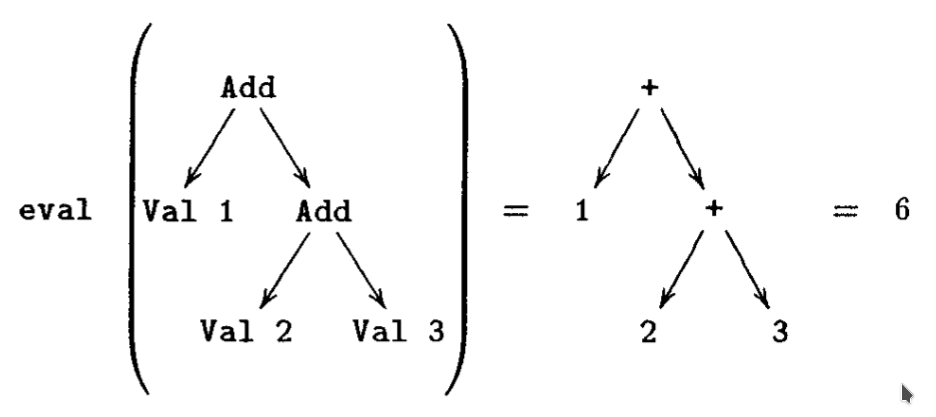
\includegraphics[width=0.6\textwidth]{figs/eval-prog}
    \caption{Денотационная семантика определяет смысл синтаксических конструкций через операции над доменом~\cite{hutton1998fold}.}
    \label{fig:eval-prog}
\end{figure}

Другим популярным стилем описания семантики является \vocab{операционная семантика}, которая представляет смысл программы в виде последовательности шагов вычислений.
Это может быть как последовательное переписывание самого выражения, так и переписывание состояния некоторой абстрактной машины.
Операционная семантика, в свою очередь, задаётся как развёртка (или анаморфизм~\ref{subsubsec:recursion-schemas}) последовательности шагов вычисления из программы.
Тут отчётливо видна некоторая двойственность между денотационной и операционной семантиками~\cite{hutton1998fold}.

\subsubsection{Встроенные доменно-специфичные языки (eDSL)} \label{subsubsec:edsl}

Обсуждение терминологии и сравнение подходов к построению DSL можно найти в~\cite{gibbons2013functional}.
Краткое описание терминов --- в конспекте курса Language Engineering~\cite{languageEngineering}.

Под \vocab{доменно-специфичными языками (domain specific languages, DSL)}\footnote{\url{https://en.wikipedia.org/wiki/Domain-specific_language}} часто понимают специализированные языки для конкретных предметных областей, например, запросов к БД или форматирования документов.
Как правило, такие языки не являются полными по Тьюрингу.

В этом курсе, однако, мы будем считать доменно-специфичным языком любую доменно-специфичную специализацию языка общего назначения\footnote{\url{https://en.wikipedia.org/wiki/Language-oriented_programming}, на русскоязычную страницу тоже следует заглянуть.}.
Это следует из того соображения, что код должен читаться как грамотным проза с уместным словоупотреблением, предоставляющая читателю только необходимое количество подробностей, скрывая несущественное за умолчаниями и терминологией.
В извечной борьбе со сложностью, мы стремимся к такому коду, строя башню из DSL\@.

\vocab{Самостоятельные доменно-специфичные языки (standalone domain specific languages)} --- языки, имеющие свой собственный конкретный синтаксис, а так же инструменты программирования (IDE, исполняющая среда\ldots).
Примеры: SQL, AWK, Antlr\ldots

\vocab{Встроенные доменно-специфичные языки (embedded domain specific languages, eDSL)} --- языки, пользующиеся поддержкой инфраструктуры других языков.
Обычно реализуются как библиотеки для программ на уже существующем языке общего назначения.
Не имеют полностью собственного синтаксиса.
Примеры: ORM, функции обработки строк, библиотека парсер-комбинаторов\ldots

\vocab{Deep eDSL} --- термы на таком языке строят дерево абстрактного синтаксиса для дальнейшей интерпретации:
\begin{minted}{haskell}
    value :: Env -> Int
    value = eval $ Const 1 `Plus` Var "x"
\end{minted}

Можно заметить, что промежуточное дерево, которое получается, нас, как правило, не интересует.
Нам важно только получить элемент домена, которым мы уже умеем пользоваться непосредственно.
\vocab{Shallow eDSL} минуют стадию построения дерева и сразу строят значение в семантическом домене: % todo переделать пример под контекст
\begin{minted}{haskell}
    cnst :: Int -> (Env -> Int)
    cnst x _ = x

    var :: String -> (Env -> Int)
    var name env = env ! name

    plus :: (Env -> Int) -> (Env -> Int) -> (Env -> Int)
    plus l r env = l env + r env

    value :: Env -> Int
    value = cnst 1 `plus` var "x"
\end{minted}

Интерпретаторы часто называют \vocab{наблюдателями (observers)}, которые анализируют термы и дают им некоторый смысл~\cite{gibbons2013functional}.
Можно заметить, что для deep eDSL можно написать сколь угодно много различных наблюдателей.
Однако в случае shallow embedding наблюдатели всегда \texttt{id}.
Мы будем обсуждать возможные решения этой проблемы в разделе~\ref{sec:wonder-interpreters}.

Введём ещё одно важное понятие.
\vocab{Meta-circular интерпретатор}\footnote{\url{https://en.wikipedia.org/wiki/Meta-circular_evaluator}}~--- это интерпретатор, определяющий конструкции определяемого языка через конструкции мета-языка~\cite{reynolds1972definitional}.
Например:
\begin{minted}{haskell}
    interpret term = case term of
      App f t -> (interpret f) (interpret t)
      If c t e -> if interpret c then interpret t else interpret e
      ...
\end{minted}

Свойства мета-языка в таком случае во многом определяют свойства объектного~\cite{reynolds1972definitional,reynolds1998definitional}.
Мы будем в этом курсе стремиться как можно более переиспользовать возможности мета-языка.

\begin{task}
    Предположите, какие свойства наследует определяемый язык.
\end{task}

% todo ссылка вперёд

\subsubsection{Пример: библиотека Accelerate}

Интересным примером встроенного языка, находящегося где-то между deep и shallow является библиотека Accelerate\footnote{\url{https://hackage.haskell.org/package/accelerate}}~\cite[глава 6]{marlow2011parallel}.
Она позволяет на Haskell описать вычисления, которые будут исполняться на GPU\footnote{Другой подход: \href{https://youtu.be/6c0DB2kwF_Q?si=-nB7AkCsDWB_Q-hy}{Java code reflection}, чтобы в рантайме извлекать модель кода. Однако, такой подход не предоставляет статически гарантий программисту и требует глубогоко внедрения в мета-язык.}.

Чтобы исполнить что-то на GPU нужно породить и скомпилировать код на Cuda.
Таким образом, Accelerate должен быть deep embedding, чтобы иметь дерево вычисления, чтобы его транслировать в Cuda наиболее эффективным образом.

В то же время описывать численные вычисления как дерево крайне неудобно.
Неплохо было бы иметь привычные операторы и функции высших порядков для работы с массивами на GPU\@.
Поэтому Accelerate предоставляет на самом деле shallow интерфейс для построения деревьев.

Так, для деревьев выражений определена реализация численных классов типов, например, \mintinline{haskell}|Num|, где операции просто достраивают дерево.
Функции высших порядков реализованы примерно с помощью техники, которую мы будем обсуждать в~\ref{subsec:first-class-functions}. % todo fix ref

% todo investigate actual HOF implementation
% todo примеры программ с Accelerate

\subsection{Expression problem} \label{subsec:expression-problem}

\vocab{Expression problem}\footnote{\url{https://en.wikipedia.org/wiki/Expression_problem}} или \vocab{проблема выразительности} --- это некоторый критерий выразительности языка программирования, сформулированный Wadler'ом в 1998\footnote{\url{https://homepages.inf.ed.ac.uk/wadler/papers/expression/expression.txt}}.
Ставится вопрос: насколько легко расширять синтаксис встроенного языка и добавлять новые интерпретации?
Иначе говоря, насколько легко добавлять новые разновидности данных и методы обработки.

Под ``легкостью'' подразумевается локальность: нужно ли править различные куски кода для этого.
Например, если синтаксис языка задан обычным алгебраическим типом данных, то добавить новую интерпретацию ``легко''~--- просто добавить новую рекурсивную функцию, а добавить новую синтаксическую конструкцию~--- ``сложно''~--- нужно изменить все интерпретаторы:
\begin{minted}{haskell}
    data Expr
      = Const Int
      | Plus Expr Expr -- добавляем

    eval :: Expr -> Int
    eval = \case Const x -> x; Plus l r -> eval l + eval r

    show :: Expr -> String
    show = \case Const x -> show x; Plus l r -> show l ++ " + " ++ show r
\end{minted}

Если язык задан с помощью наследования, то, наоборот, расширить синтаксис легко --- добавить новый класс, а добавить интерпретацию сложно --- добавить реализацию метода в каждом классе:
\begin{minted}{kotlin}
    interface Lang {
        fun eval(): Int
        fun show(): String
    }
    class Const(val x: Int) : Lang {
        override fun eval() = x
        override fun show() = x.toString()
    }
    class Plus(val l: Lang, val r: Lang) : Lang {
        override fun eval() = l.eval() + r.eval()
        override fun show() = "$l + $r"
    }
\end{minted}

Оказывается, существуют подходы, позволяющие добиться ``лёгкости'' по обоим измерениям.
Мы уделим им много внимания в этом курсе.

Действительно, как мы обсуждали ранее~\ref{subsec:interpreters-tower}, программы представляют собой серию интерпретаторов.
Для всё той же борьбы со сложностью, важно уметь описывать эти интерпретаторы модульно --- задавать части языков отдельно друг от друга, и собирать нужные языки по месту из готовых блоков.
Это помогает составлять программы из простых переиспользуемых компонент, каждая из которых имеет чёткую зону ответственности.

Expression problem возникала и решалась много раз: expression problem, stable denotations, extensible (modular) interpreters.
Прошло немало времени, пока не возникло понимание, что всё это об одном и том же\footnote{\url{https://okmij.org/ftp/Computation/having-effect.html}}.

% todo Independently Extensible Solutions to the Expression Problem
